\section{Ontwerp}
Voor dit onderzoek heb ik een virtuele omgeving ontworpen met meer dan 48m$^2$
aan bewandelbare ruimte, de proefpersoon kan deze omgeving volledig verkennen en
toch in een 3 m x 4 m tracking area blijven.

Deze virtuele omgeving bestaat uit een lange gang met drie kantoren en een 
uitgang er direct aan verbonden. De kantoren zijn zo ontworpen dat het mogelijk 
is om de deur te verplaatsen wanneer de proefpersoon deze niet in het zicht
heeft. De gang zelf is 1 meter breed met een arbitraire lengte zodat deze
oneindig lang lijkt. De kantoren zijn allemaal ontworpen om 3 m x 3 m te zijn.

Bij het betreden van de virtuele omgeving staat de proefpersoon aan het begin van
de gang, aan de rechtermuur zijn 4 deuren te zien, 80 cm breed met 80 cm er
tussen.

Bij het betreden van het kantoor en het sluiten van de blinden wordt de hele 
gang naar achter verschoven zodat de deur nu aan de andere kant van de kamer 
staat zoals ge\"illustreerd in figuur \ref{fig:verandering}, na het verlaten van 
het kantoor staat de proefpersoon weer op de exacte locatie waar hij begonnen is.
Wegens de beweging van de gang wordt er hier de illusie gecre\"eerd dat men
verder in de gang staat dan eerst. De proefpersoon kan dan de deur van het 
kantoor sluiten om de volgende deur te openen. Dit geheel wordt drie keer 
herhaald.

De beweging van de gang wordt teweeg gebracht door een transformatie in de
positie te laten gebeuren na het triggeren van de knop, wegens de gekozen hoek is
de deur hier nooit voor in beeld.

\begin{figure}[h!]
    \centering
    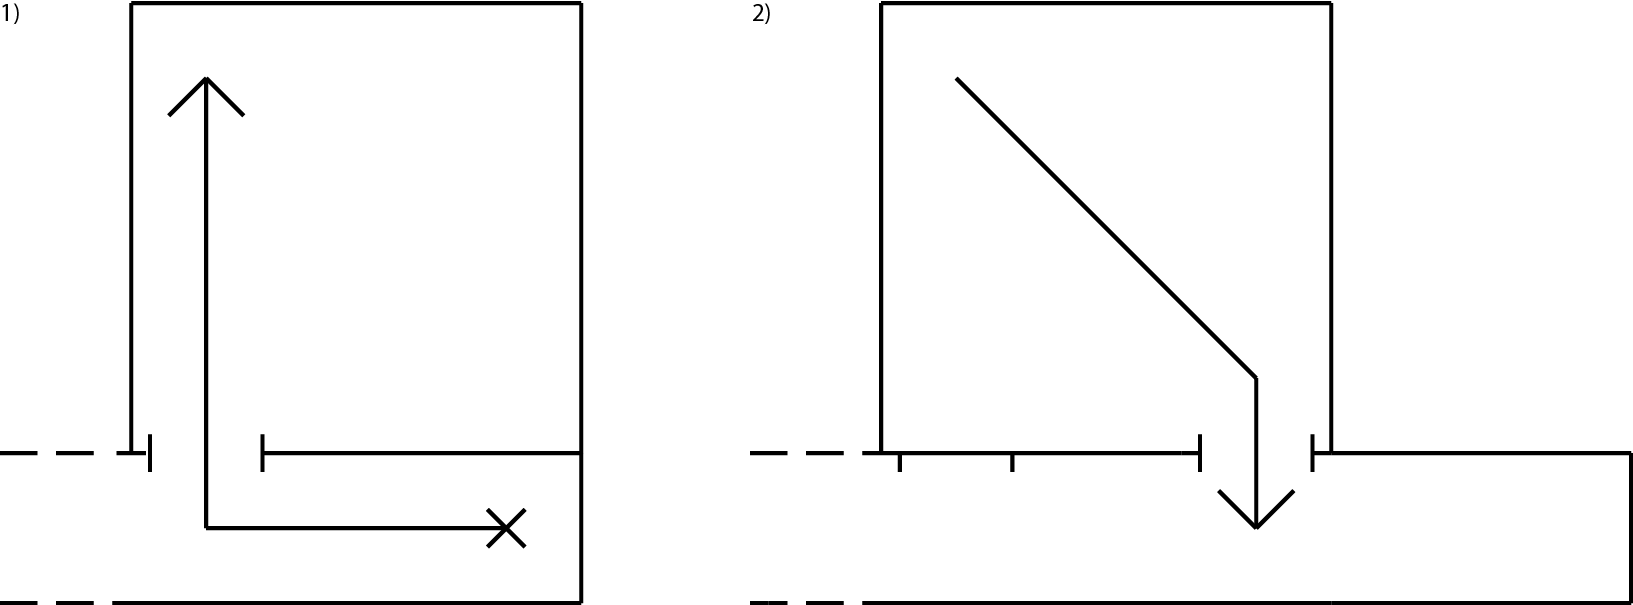
\includegraphics[width=\textwidth]{verandering}
    \caption{Verandering van de omgeving.}
    \label{fig:verandering}
\end{figure}

Om wat vari\"eteit te behouden zijn de drie kantoren, zoals ge\"illustreerd 
in figuur \ref{fig:kantoren}, lichtjes verschillend ontworpen. Enkel de knop om 
de blinden te sluiten en het fotokader er boven staat in ieder kantoor op 
dezelfde plaats.

\begin{figure}[h!]
    \centering
    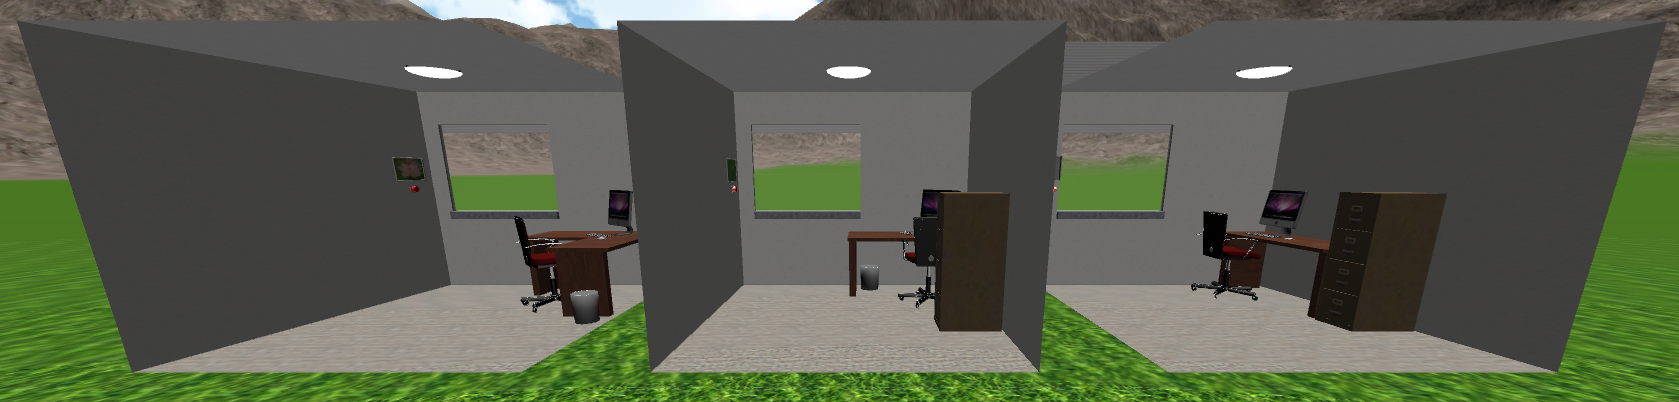
\includegraphics[width=\textwidth]{offices}
    \caption{De drie kantoren.}
    \label{fig:kantoren}
\end{figure}

De vierde kamer dient enkel als markering van het einde, bij het betreden van
deze kamer gaan de lichten langzaam uit.

Om een kleine hoeveelheid ruimte rondom de tracking area over te houden heb ik
een constante factor van 1.1 op de bewegingssnelheid toegepast daar dit klein 
genoeg is om onmerkbaar te zijn\cite{steinicke09}.

Wegens de manier waarop dit systeem werkt is het onmogelijk om een grondplan te
tekenen dat overeen komt met de realiteit, in figuur \ref{fig:plan} is te zien
wat het beoogde mentale vloerplan is van de testpersonen.

\begin{figure}[h!]
    \centering
    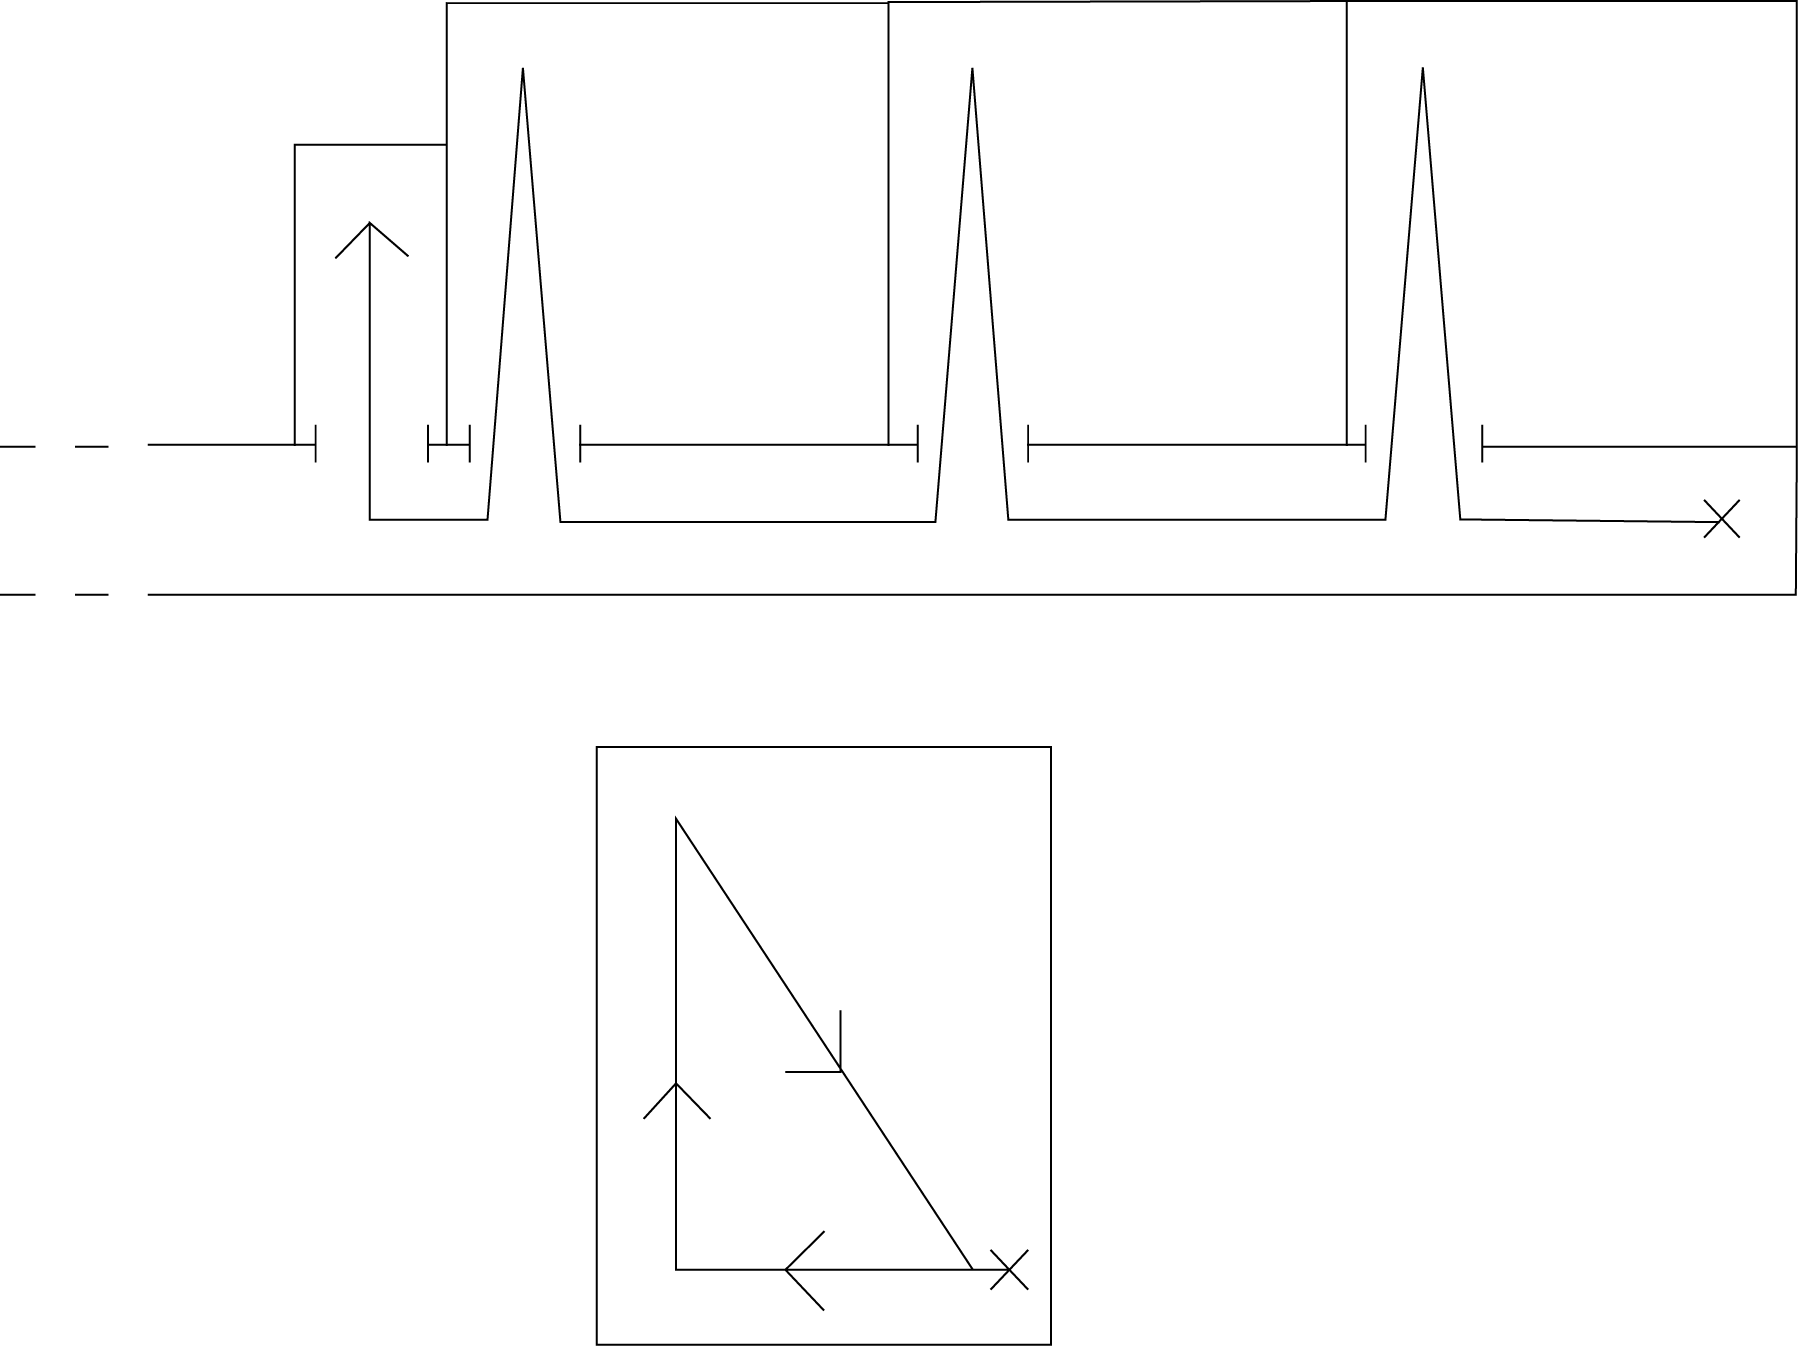
\includegraphics[width=\textwidth]{plan}
    \caption{Mentaal grondplan van de virtuele omgeving.}
    \label{fig:plan}
\end{figure}


\section{Implementatie}
\subsection{Engine}
Voor de implementatie van de virtuele omgeving heb ik er voor gekozen om met de
Unity engine te werken. Ik heb deze keuze gemaakt omdat de Unity engine relatief
eenvoudig is om mee te werken en mij meer tijd over laat om te werken aan de
benodigde algoritmen.

Voor het ontwerp van de omgeving heb ik gebruik gemaakt van de Blender 3d
editor, wegens eerdere ervaring met deze editor.

\subsection{Tracking}
Voor integratie met het trackingsysteem heb ik gebruik gemaakt van de gratis
editie van de MiddleVR middleware. Deze maakt het mogelijk om via het VRPN
protocol te communiceren met de tracking server.

MiddleVR geeft ook toegang tot ``virtual trackers'' waarmee men de data van een
tracker kan transformeren. Het resultaat hiervan is dat ik de pitch en de roll
van de HMD heb kunnen gebruiken, en de yaw van het camera tracking systeem. Dit
omdat de HMD een kleine hoeveelheid ``yaw drift'' heeft, en dit zou kunnen zorgen
voor botsingen met de fysieke omgeving.

Ik heb dit systeem ook gebruikt om de trillingen in de gerapporteerde yaw van het
trackingsysteem te verminderde, door een gemiddelde van twee metingen te
gebruiken. Daar de ``framerate'' van het systeem voldoende is, heeft dit bijna 
geen effect op de latency van de bewegingen.

In de praktijk werkt dit door te werken met het gemiddelde van de vorige meting
en de nieuwe meting in plaats van met de rauwe meting te werken.

Aan de serverkant heb ik gebruik gemaakt van de OptiTrack:Motive software om de
VRPN data te broadcasten.

\subsection{Hardware}
Om een vloeiende werking te verzekeren werd de virtuele omgeving gedraaid op een
Apple MacBook Pro (13", midden 2012) met een 2,5 GHz Intel Core i5 processor, 
8 GB 1333 MHz DDR3 RAM geheugen en een Intel HD Graphics 4000 GPU.

Het beeld werd getoond op een Oculus Rift (Devkit 1) aan 60 fps voor beide ogen.
Deze HMD heeft een diagonale FoV van 110\textdegree{} en vult hierdoor bijna het
hele zicht van de proefpersonen voor een maximale immersie.

Tracking van positie en rotatie in 3 assen werd gedaan door een 6 camera
OptiTrack systeem rondom een 3 m x 4 m omgeving.

Om gebruikersinvoer te voorzien heb ik gewoon een bluetooth muis gebruikt, zodat
de proefpersoon op eender welke knop kon klikken om het object voor hem te
activeren.